
%(BEGIN_QUESTION)
% Copyright 2010, Tony R. Kuphaldt, released under the Creative Commons Attribution License (v 1.0)
% This means you may do almost anything with this work of mine, so long as you give me proper credit

Decode the following serial data streams, each one encoded using a different method:

$$
\includegraphics[width=15.5cm]{i02919x02.eps}$$

\vskip 30pt

$$
\includegraphics[width=15.5cm]{i02919x03.eps}$$

\vskip 30pt

\vskip 20pt \vbox{\hrule \hbox{\strut \vrule{} {\bf Suggestions for Socratic discussion} \vrule} \hrule}

\begin{itemize}
\item{} Assuming a common time scale for both data streams shown, which of the two has the highest {\it bit rate}?
\item{} Assuming a common time scale for both data streams shown, which of the two has the highest {\it baud rate}?
\end{itemize}

\underbar{file i02919}
%(END_QUESTION)





%(BEGIN_ANSWER)

$$\includegraphics[width=15.5cm]{i02919x01.eps}$$

\vskip 10pt

$$\includegraphics[width=15.5cm]{i02919x04.eps}$$

%(END_ANSWER)





%(BEGIN_NOTES)

%INDEX% Electronics review: Manchester encoding
%INDEX% Electronics review: FSK encoding

%(END_NOTES)

